\section{Complessità}

\subsection{Notazione asintotica}
Quando scriviamo un algoritmo, per calcolarne il costo, bisogna fare una serie di assunzioni sulla macchina astratta su cui lavoriamo:
\begin{itemize}
	\item L'accesso alle celle di memoria avviene in tempo costante.
	\item Le operazioni elementari avvengono in tempo costante:
	\begin{itemize}
		\item Operazioni aritmetiche e logiche della ALU
		\item Gli assegnamenti
		\item I controlli del flusso (salti, assegnamento al registro PC)
	\end{itemize}
	
\end{itemize}
Per calcolare il costo degli algoritmi si possono utilizzare due modelli:
\begin{enumerate}
	\item \textbf{Word model}: tutti i dati occupano solo una cella di memoria.
	\item \textbf{Bit model}: unità elementare di memoria \emph{bit}, si usa quando le grandezze sono troppo grandi.
\end{enumerate}

\noindent Esistono una serie di parametri da \textbf{analizzare} quando scriviamo una algoritmo. Essi permettono di garantire il suo corretto funzionamento e la sua ottimizzazione. Sono i seguenti:
\begin{itemize}
	\item \textbf{Complessità}: ovvero l'analisi dell'utilizzo delle risorse: 
	\begin{itemize}
		\item tempo di esecuzione
		\item spazio di memoria per i dati in ingresso e in uscita. Viene rappresentato astrattamente dal numero di celle di memoria (word model)
		\item banda di comunicazione (per esempio nel caso il calcolo sia distribuito)
	\end{itemize}
	Non sarà quasi mai possibile avere un programma che è sia efficiente in termini di tempo che in di spazio (\emph{coperta corta}).
	\item \textbf{Correttezza}: Indica se l'algoritmo fa quello per cui è stato progettato. Si esegue in due modi:
	\begin{itemize}
		\item \underline{dimostrazione formale} la quale permette di dimostrare la correttezza risolvendo tutte le istanze del problema
		\item \underline{ispezione formale} nella quale si usano metodi come il \textbf{testing} o il \textbf{profiling}. Il primo prevede di provare il programma nelle situazioni critiche, il secondo analizza il tempo che la CPU impiega per elaborare una determinata parte del programma.
	\end{itemize}
	\item \textbf{Semplicità}: Indica se l'algoritmo è facile da capire e manutenere. Un algoritmo è semplice quando usa identificatori significativi, quando è ben commentato, se usa strutture dati adeguate e se rispetta gli standard.
\end{itemize}

\begin{definition}[Complessità di un problema]
	La complessità di un problema $P$ è la complessità del miglior algoritmo $A$ che lo risolve.
\end{definition}
Per trovare la complessità del problema partiamo dal fatto che, dato un algoritmo $A$, la complessità di $A$ determina un limite superiore alla complessità di $P$ (cioè quando si verifica il caso peggiore uso $A$ per risolvere $P$).\\
Se riusciamo a determinare un limite inferiore $g(n)$ per $P$, per ogni algoritmo $A$ che risolve $P$ ho che $A \in \Omega(g(n))$, dove $g(n)$ è il minimo numero di operazione che posso impiegare per risolvere $P$. Quindi possiamo dire che:
\begin{equation}
	A \in \Theta(g(n)) \Longrightarrow A \text{ ottimo} \footnote{Ricorda che dire che $A \in \Theta(g(n))$ vuol dire che $A \in O(g(n))$ e $A \in \Omega(g(n))$}
\end{equation}
Per fare ciò bisogna anche andare a calcolare il limite inferiore del caso pessimo, e ciò è possibile tramite 3 metodi: la \textbf{dimensione dei dati}, gli \textbf{eventi contabili} e gli \textbf{alberi decisionali}.

\begin{itemize}
	\item \textbf{Dimensione dei dati}: Se la soluzione di un problema richiede l'esame di tutti i dati in input, allora $\Omega(n)$ è un limite inferiore. \emph{E.g. sommare tutti gli elementi di un array.}
	\item \textbf{Eventi contabili}: se la soluzione di un problema richiede la ripetizione di un certo evento, allora il numero di volte che l'evento si ripete (moltiplicato per il suo costo) è un limite inferiore.
	\item \textbf{Alberi di decisione}: sono alberi in cui
	\begin{itemize}
		\item ogni nodo non foglia effettua un test su un attributo
		\item ogni arco uscente da un nodo è un possibile valore dell'attributo
		\item ogni nodo foglia assegna una classificazione
	\end{itemize}
	Si applica a problemi risolubili attraverso sequenze di decisioni che via via riducono lo spazio delle soluzioni.
	\begin{figure}[!h]
		\centering
		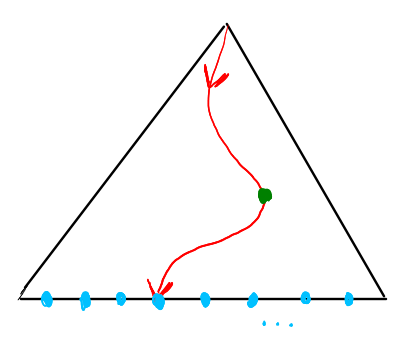
\includegraphics[width=5cm]{images/albero-decisionale.png}
		\caption{Albero decisionale}
	\end{figure}
	\\In figura vediamo che dalla situazione iniziale, tramite un \color{red} percorso radice-foglia \color{black} (ovvero un'esecuzione dell'algoritmo), otteniamo una tra le possibili \color{blue} soluzioni \color{black}  (foglie) passando per diverse \color{green} decisioni \color{black} (nodi interni).
	\begin{note}
		Alcune formule importanti per gli alberi:
		\begin{itemize}
			\item  \textbf{Foglie}: $n^d$
			\item \textbf{Profondità} $d \leq \log_n$ foglie (è esattamente uguale solo se l'albero è completo)
			\item \textbf{Nodi}: $n^{d+1}-1$			
		\end{itemize}
	\end{note}
	\begin{example} Ricerca binaria di un elemento $k$ in un array $A$ di $n$ elementi. Ogni confronto tra $k$ e $A[cen]$ può generare 3 possibili risposte:
		\begin{itemize}
			\item $k < A[cen]$ ramo sinistro
			\item $k == A[cen]$ ramo centrale
			\item $k > A[cen]$ ramo destro
		\end{itemize}
	Abbiamo quindi che ogni confronto apre 3 possibili vie e dopo $i$ confronti avremo $3^i$ vie. Le possibili soluzioni sono $n+1$ ($k$ può essere in ognuna delle $n$ posizioni o non esserci). Avremo quindi:
	\begin{equation}
		3^i \geq n+1 > n \implies \text{binSearch} \in \Omega(\log_n)
	\end{equation}
		
	\end{example}
\end{itemize}

\subsection{Big-O notation}
La notazione Big-O ha molteplici scopi nella scrittura di un algoritmo.
\begin{itemize}
	\item Serve a rappresentare la complessità relativa di un algoritmo.
	\item Descrive le prestazioni di un algoritmo e come queste scalano al cresce dei dati in input.
	\item Descrive un limite superiore al tasso di crescita di una funzione ed è il caso peggiore.
\end{itemize}

\subsubsection{Limite superiore asintotico}
\begin{definition}[Limite superiore asintotico]
	Il limite superiore asintotico \footnote{\emph{Asintotico} indica che la definizione deve essere valida solo da un certo punto in poi scelto arbitrariamente.} si definisce come:
	\begin{equation}
		O(g(n)) = \{f(n) \mid \exists c, n_0 > 0 . \forall n > n_0, 0 \leq f(n) \leq c \cdot g(n)\}
	\end{equation}
\end{definition}
\noindent Si scrive come $f(n) \in O(g(n))$ oppure $f(n) = O(g(n))$ e si legge $f(n)$ è nell'ordine $O$ grande di $g(n)$.
\begin{example}
	Esempio di calcolo del limite superiore asintotico
\end{example}
\begin{wrapfigure}[7]{l}{8cm}
	\vspace{-15pt}
	\centering
	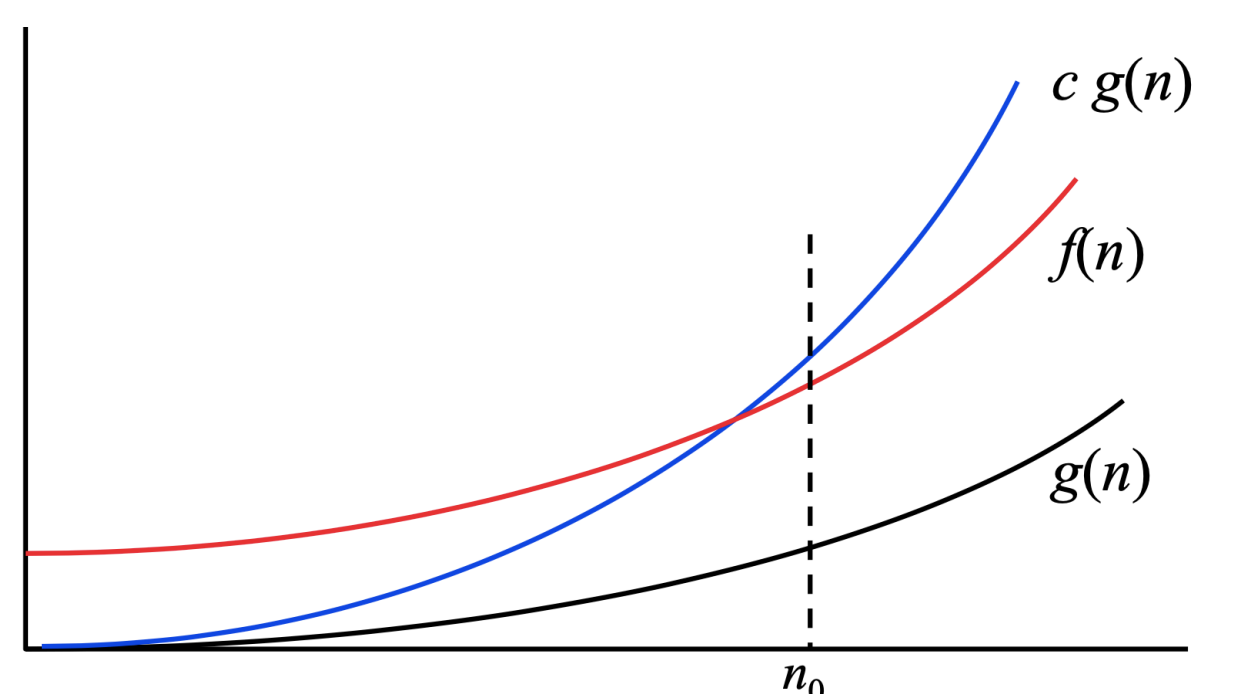
\includegraphics[width=6cm]{images/limite-superiore-asintotico.png}
	\vspace{-5pt}
	\caption{Limite superiore asintotico}
\end{wrapfigure}
Prendiamo due funzioni e determiniamo i punti $n_0$ e $c$ per cui è soddisfatta la definizione.
\begin{center}
	\vspace{-5pt}
	$f(n) = 3n^2 + 5$\hspace{30pt}$g(x)=n^2$
\end{center}
Stabiliamo un $c = 4$ e $n_0 = 3$.
\begin{enumerate}
	\item $4 \cdot g(n) = 4n^2 = 3n^2 + n^2 $
	\item $3n^2 + n^2 \geq 3n^2 + 9 $ (per ogni $n \geq 3$)
	\item $3n^2 + 9 > 3n^2+5 \Longrightarrow 4 \cdot g(n) > f(n)$
\end{enumerate}

\begin{note}
	Abbiamo disegnato solo il primo quadrante perché sia i dati in input che le operazioni da eseguire saranno sempre in numero positivo.
\end{note}

\subsubsection{Limite inferiore asintotico}
\begin{definition}[Limite inferiore asintotico]
	Il limite inferiore asintotico si definisce come:
	\begin{equation}
		\Omega(g(n)) = \{f(n) \mid \exists c, n_0 > 0 . \forall n > n_0, 0 \leq c \cdot g(n) \leq f(n) \}
	\end{equation}
\end{definition}
\noindent Si scrive come $f(n) \in \Omega(g(n))$ oppure $f(n) = \Omega(g(n))$ e si legge $f(n)$ è nell'ordine $\Omega$ grande di $g(n)$. Indica che quell'algoritmo non potrà mai fare di meglio.
\begin{example}
	Esempio di calcolo del limite inferiore asintotico. Prendiamo due funzioni e determiniamo i punti $n_0$ e $c$ per cui è soddisfatta la definizione.
\end{example}
\begin{wrapfigure}[6]{r}{8cm}
	\vspace{-15pt}
	\centering
	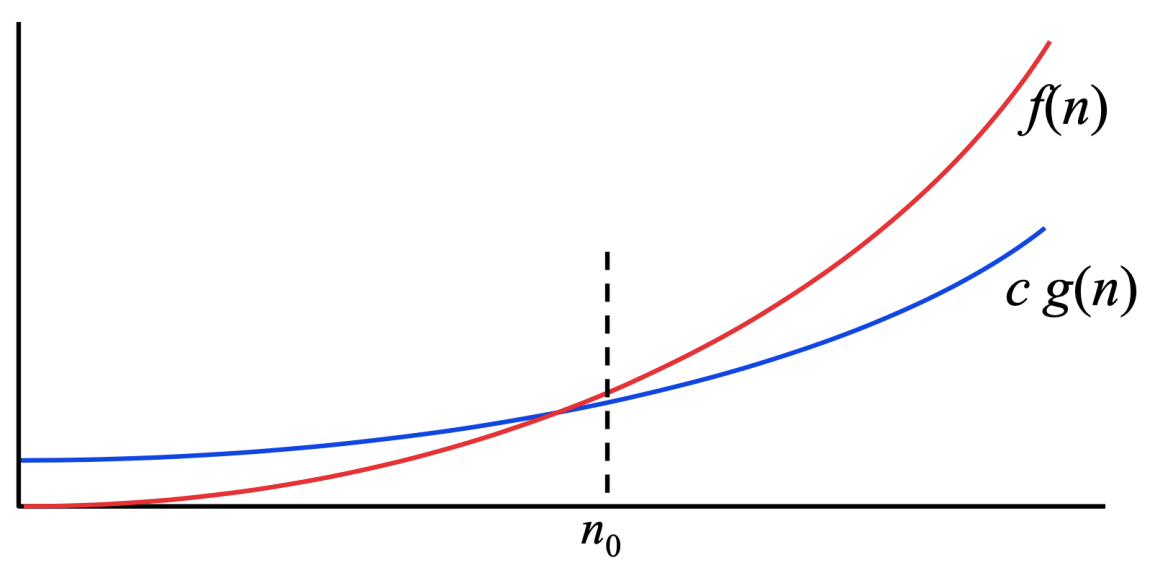
\includegraphics[width=6cm]{images/limite-inferiore-asintotico.png}
	\vspace{-5pt}
	\caption{Limite superiore asintotico}
\end{wrapfigure}

$f(n) = \frac{n^2}{2}-7$ \: \: \: $g(x)=n^2$\\
Stabiliamo un $c = \frac{1}{4}$ e $n_0 = 6$.
\begin{enumerate}
	\item $\frac{1}{4} \cdot g(n) = \frac{n^2}{4} = \frac{n^2}{2} - \frac{n^2}{4}$
	\item $\frac{n^2}{2} - \frac{n^2}{4} \leq \frac{n^2}{2} - 9 $ (per ogni $n \geq 6$)
	\item $\frac{n^2}{2} - 9 > \frac{n^2}{2}-7 \Longrightarrow \frac{1}{4} \cdot g(n) < f(n)$
\end{enumerate}

\subsubsection{Limite asintotico stretto}
\begin{definition}[Limite asintotico stretto]
	Il limite asintotico stretto si definisce come:
	\begin{equation}
		\Theta(g(n)) = \{f(n) \mid \exists c_1, c_2, n_0 > 0 . \forall n > n_0, 0 \leq c_1 \cdot g(n) \leq f(n) \leq c_2 \cdot g(n) \}
	\end{equation}
\end{definition}
\begin{wrapfigure}[5]{l}{8cm}
	\vspace{-10pt}
	\centering
	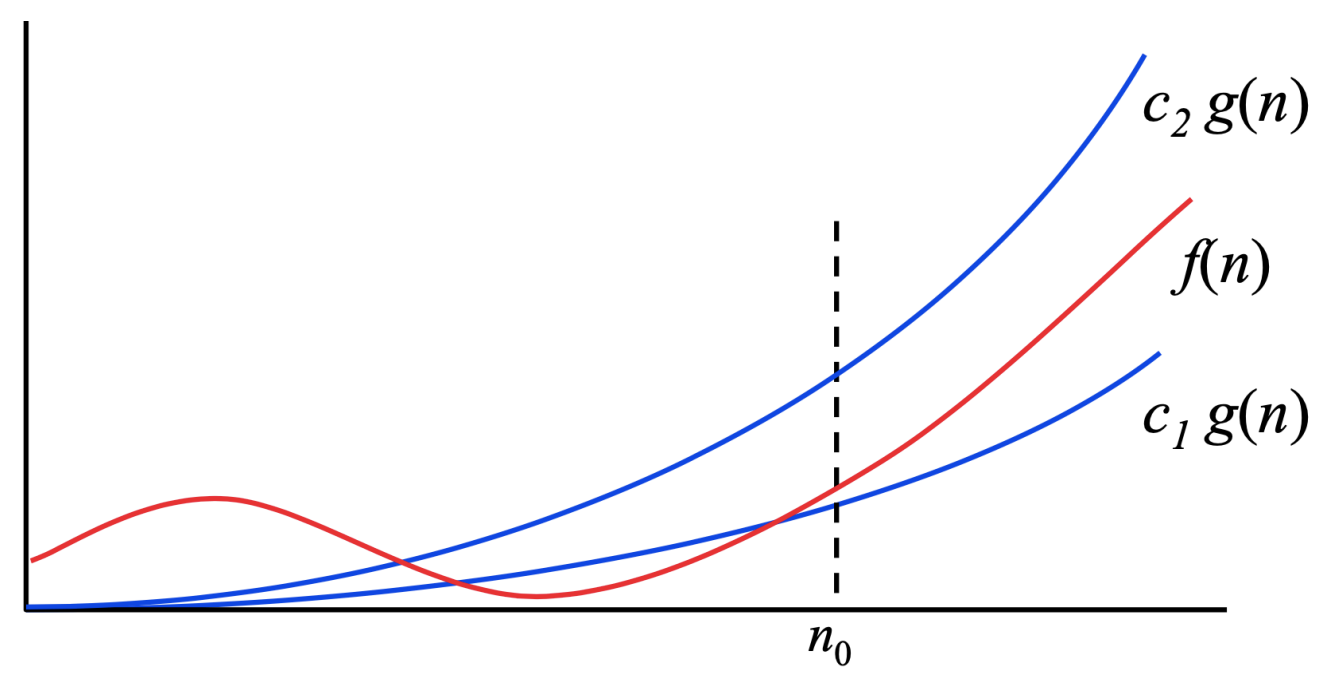
\includegraphics[width=6cm]{images/limite-asintotico-stretto.png}
	\vspace{-5pt}
	\caption{Limite asintotico stretto}
\end{wrapfigure}
Si scrive come $f(n) \in \Theta(g(n))$ oppure $f(n) = \Theta(g(n))$ e si legge $f(n)$ è nell'ordine $\Theta$ grande di $g(n)$.\\\\

\vspace{55pt}
Dalla definizione deriva che:
\begin{equation}
	f(n) \in \Theta(g(n)) \Longleftrightarrow f(n) \in \Omega(g(n)) \land f(n) \in O(g(n))
\end{equation}

\subsubsection{Teoremi sulla notazione asintotica}
\begin{theorem}
	Per ogni $f(n)$ e $g(n)$ vale che:
	\begin{enumerate}
		\item $f(n) = O(g(n)) \Longleftrightarrow g(n) = \Omega(f(n))$
		\item Se $f_1(n) = O(f_2(n)) \land f_2(n) = O(f_3(n)) \Longrightarrow f_1(n) = O(f_3(n))$
		\item Se $f_1(n) = \Omega(f_2(n)) \land f_2(n) = \Omega(f_3(n)) \Longrightarrow f_1(n) = \Omega(f_3(n))$
		\item Se $f_1(n) = \Theta(f_2(n)) \land f_2(n) = \Theta(f_3(n)) \Longrightarrow f_1(n) = \Theta(f_3(n))$
		\item Se $f_1(n) = O(g_1(n)) \land f_2(n) = O(g_2(n)) \Longrightarrow O(f_1(n) + f_2(n)) = O(max\{g_1(n),g_2(n)\})$
		\item Se $f(n)$ è un polinomio di grado $d \Longrightarrow f(n) = \Theta(n^d)$
	\end{enumerate}
\end{theorem}

\subsubsection{Limite superiore asintotico non stretto}
\begin{definition}[Limite superiore asintotico non stretto]
	Il limite superiore asintotico non stretto si definisce come:
	\begin{equation}
		o(g(n)) = \{f(n) \mid \forall c \exists n_0 > 0 . \forall n > n_0, 0 \leq f(n) \leq c \cdot g(n) \}
	\end{equation}
\end{definition}
\noindent Si scrive come $f(n) \in o(g(n))$ oppure $f(n) = o(g(n))$ e si legge $f(n)$ è nell'ordine $o$ piccolo di $g(n)$.\\
$f(n)$ è limitata superiormente da $g(n)$, ma non la raggiunge mai.\\
\begin{wrapfigure}[7]{l}{7cm}
	\vspace{-15pt}
	\centering
	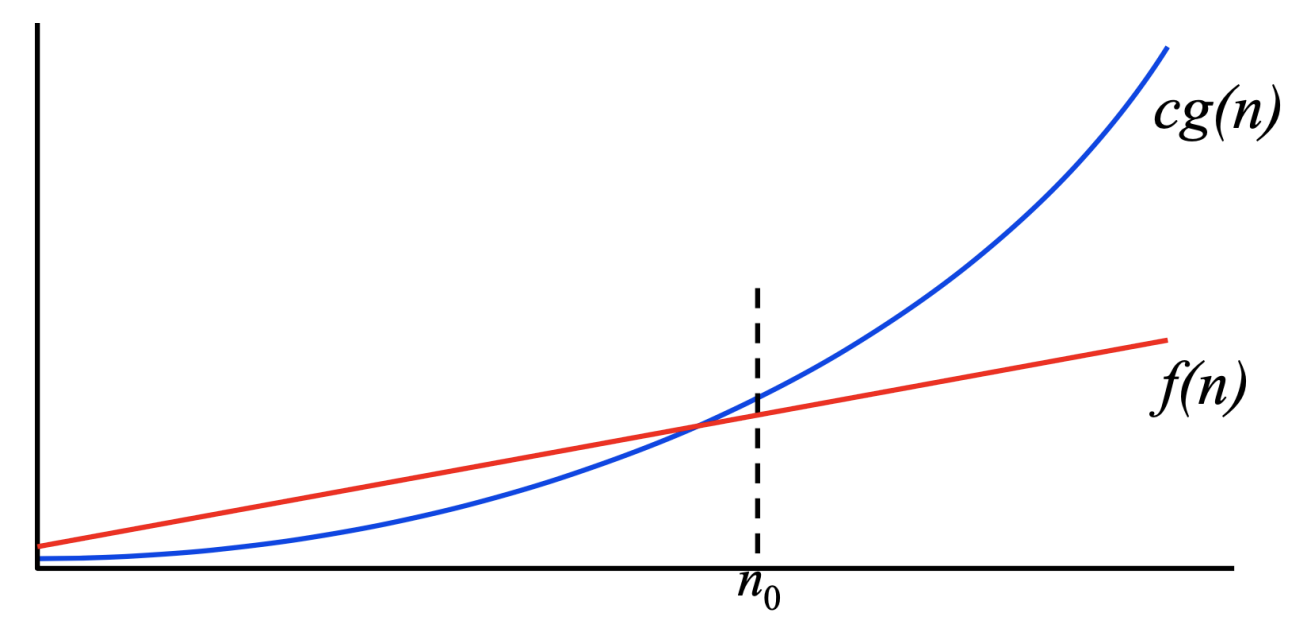
\includegraphics[width=6.5cm]{images/limite-superiore-asintotico-non-stretto.png}
	\vspace{-5pt}
	\caption{Limite superiore non stretto}
\end{wrapfigure}

\vspace{-15pt}
E immediato dalla definizione che:
\begin{center}
	$o(g(n)) \Longrightarrow O(g(n))$
\end{center}
Non vale il contrario: 
\begin{center}
	$2n^2 \in O(n^2) \land 2n^2 \notin o(n^2)$
\end{center}
Definizione alternativa:
\begin{center}
	$f(n) \in o(g(n)) \Longleftrightarrow \lim\limits_{n\to \infty}\frac{g(n)}{f(n)} = \infty$
\end{center}

\subsubsection{Limite inferiore asintotico non stretto}
\begin{definition}[Limite inferiore asintotico non stretto]
	Il limite inferiore asintotico non stretto si definisce come:
	\begin{center}
		$\omega(g(n)) = \{f(n) \mid \forall c \: \exists n_0 > 0 . \forall n > n_0, 0 \leq c \cdot g(n) \leq f(n) \}$
	\end{center}
\end{definition}
\noindent Si scrive come $f(n) \in \omega(g(n))$ oppure $f(n) = \omega(g(n))$ e si legge $f(n)$ è nell'ordine $\omega$ piccolo di $g(n)$.\\
$f(n)$ è limitata inferiormente da $g(n)$, ma non la raggiunge mai.\\
\begin{wrapfigure}[7]{l}{7cm}
	\vspace{-15pt}
	\centering
	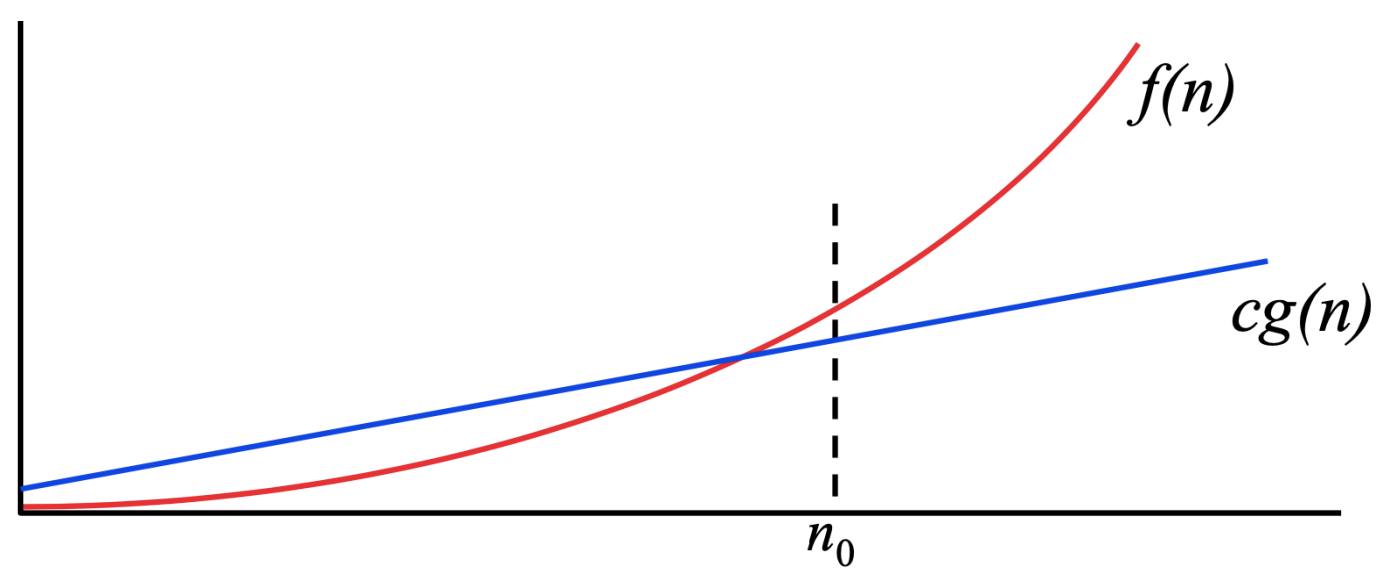
\includegraphics[width=6.5cm]{images/limite-inferiore-asintotico-non-stretto.png}
	\vspace{-5pt}
	\caption{Limite asintotico stretto}
\end{wrapfigure}

\vspace{-15pt}
E immediato dalla definizione che:
\begin{center}
	$\omega(g(n)) \Longrightarrow \Omega(g(n))$
\end{center}
Non vale il viceversa: 
\begin{center}
	$\frac{1}{5}n^2 \in \Omega(n^2) \land \frac{1}{2}n^2 \notin \omega(n^2)$
\end{center}
Definizione alternativa:
\begin{center}
	$f(n) \in \omega(g(n)) \Longleftrightarrow \lim\limits_{n\to \infty}\frac{g(n)}{f(n)} = 0$
\end{center}

\subsection{Ordinamento}
\subsubsection{Insertion sort}
\textbf{Proprietà}: al termine del passo j-esimo dell'algoritmo l'elemento j-esimo viene in inserito al posto giusto e i primi $j+1$ elementi sono ordinati.
\begin{lstlisting}[language=Javascript, caption=Algoritmo insertion sort, mathescape=true]
	insertionSort(A) =
	var j:Int = 0;
	var i:Int = 0;		$\Theta(1)$
	var k:int = 0;
	for (j=1; j<n; j++) {		$n-1$ volte
		k = A[j];
		i = j-1;		$\Theta(1)$ $n-1$ volte
		while(i >= 0 && A[i]>k) {
			A[i+1] = A[i];			$\Theta(1)$ $\sum\limits_{j=1}^{n-1} (t_j-1)$ volte
			i=i-1;
		}
		A[i+1] = k;		$\Theta(1)$ $n-1$ volte
	}
\end{lstlisting}

\begin{table}[h]
	\centering
	\begin{tabular}{ |c|c|c|c|c|c| }
		\hline
		0 & 1 & 2 & 3 & 4 & 5 \\
		\hline
		5 & 2 & 4 & 6 & 1 & 3 \\
		\hline 
		5 & 2 & 4 & 6 & 1 & 3 \\
		\hline 
		5 & 5 & 4 & 6 & 1 & 3 \\
		\hline 
		2 & 5 & 4 & 6 & 1 & 3 \\
		\hline 
		2 & 5 & 4 & 6 & 1 & 3 \\
		\hline 
		2 & 5 & 5 & 6 & 1 & 3 \\
		\hline 
		2 & 4 & 5 & 6 & 1 & 3 \\
		\hline 
		2 & 4 & 5 & 6 & 1 & 3 \\
		\hline 
		2 & 4 & 5 & 6 & 1 & 3 \\
		\hline 
	\end{tabular}
	\begin{tabular} { |c|c|c|c|}
		\hline
		j & i & k & while \\
		\hline
		0 & 0 & 0 & no \\
		\hline
		1 & 0 & 2 & si \\
		\hline
		1 & -1 & 2 & no \\
		\hline
		1 & -1 & 2 & no \\
		\hline
		2 & 1 & 4 & si \\
		\hline
		2 & 0 & 4 & no \\
		\hline
		2 & 0 & 4 & no \\
		\hline
		3 & 2 & 6 & no \\
		\hline
		3 & 2 & 6 & no \\
		\hline
	\end{tabular}
	\caption{Esempio di esecuzione}
\end{table}
\textbf{Complessità}:
\begin{equation}
	\sum\limits_{j=1}^{n-1} t_j
\end{equation}
\begin{itemize}
	\item Caso pessimo: l'array è ordinato decrescente e quindi ogni volta devo scalare l'elemento fino alla prima posizione. Abbiamo che $t_j = j$ e $\sum\limits_{j=1}^{n-1} j = \frac{n(n-1)}{2}$, quindi $O(n^2)$
	\item Caso migliore: l'array è ordinato crescente e quindi per ogni iterazione non entro nel while perché la condizione è falsa. Abbiamo $t_j = 1$ e $\sum\limits_{j=1}^{n-1} j = n-1$, quindi $O(n)$
	\item Caso medio: come il caso pessimo $O(n^2)$
\end{itemize}
\textbf{Correttezza}:
\begin{itemize}
	\item dimostro l'\textbf{invariante di ciclo} per assicurarmi che la mia proprietà venga mantenuta durante tutta l'esecuzione. Lo faccio tramite \emph{induzione}:
	\begin{itemize}
		\item Caso base: per $j=1$
		\item Hp induttiva: per $j=n'$
		\item Passo induttivo: dimostro che vale anche per $j=n'+1$
	\end{itemize}
	\item verifico la \textbf{terminazione}: il \emph{for} è eseguito esattamente $n-1$ volte e il \emph{while} al più $j-1$ volte, quindi tutte le iterazioni sono finite e l'algoritmo termina.
\end{itemize}
\textbf{Memoria impiegata}: ordina in loco quindi non usa memoria aggiuntiva.

\subsubsection{Selection sort}
\textbf{Proprietà}: al termine del passo j-esimo dell'algoritmo i primi $j+1$ elementi di A sono ordinati e contengono i $j+1$ elementi più piccoli di A.
\begin{lstlisting}[language=Javascript, caption=Algoritmo selection sort, mathescape=true]
	insertionSort(A) =
	var j:Int = 0;
	var i:Int = 0;		$\Theta(1)$
	var min:int = 0;
	for (i=0; i<n-1; i++) {		$n-1$ volte
		min = i;		$\Theta(1)$ $n-1$ volte
		for(j=i+1; j<n; j++) {
			if A[j] < A[min] {min = j};			$\Theta(1)$ $\sum\limits_{j=1}^{n-1} (t_j-1)$ volte
		}
		swap(A[i],A[min]);		$\Theta(1)$ $n-1$ volte
	}
\end{lstlisting}
\begin{table}[h]
	\centering
	\begin{tabular}{ |c|c|c|c|c|c| }
		\hline
		0 & 1 & 2 & 3 & 4 & 5 \\
		\hline
		5 & 2 & 4 & 6 & 1 & 3 \\
		\hline 
		1 & 2 & 4 & 6 & 5 & 3 \\
		\hline 
		1 & 2 & 4 & 6 & 5 & 3 \\
		\hline 
		1 & 2 & 3 & 6 & 5 & 4 \\
		\hline 
		1 & 2 & 3 & 4 & 5 & 6 \\
		\hline 
		1 & 2 & 3 & 4 & 5 & 6 \\
		\hline
	\end{tabular}
	\begin{tabular} { |c|c|c|}
		\hline
		j & i & min \\
		\hline
		0 & 0 & 0 \\
		\hline
		1 & 0 & 4 \\
		\hline
		2 & 1 & 1 \\
		\hline
		3 & 2 & 5 \\
		\hline
		4 & 3 & 3 \\
		\hline
		5 & 4 & 4 \\
		\hline
	\end{tabular}
	\caption{Esempio di esecuzione}
\end{table}
\textbf{Complessità}
%TODO Inserisci il calcolo della complessità
\begin{equation}
	\sum\limits_{j=1}^{n-1} j = \frac{n(n-1)}{2} \in O(n^2)
\end{equation}
\begin{itemize}
	\item Caso pessimo: $O(n^2)$
	\item Caso migliore: $O(n^2)$
	\item Caso medio: $O(n^2)$
\end{itemize}
\textbf{Correttezza}:
\begin{itemize}
	\item dimostro l'\textbf{invariante di ciclo} per assicurarmi che la mia proprietà venga mantenuta durante tutta l'esecuzione. Sempre tramite induzione.
	\item verifico la \textbf{terminazione} in maniera analoga all'insertion sort.
\end{itemize}
\textbf{Memoria impiegata}: ordina in loco quindi non usa memoria aggiuntiva.